\subsection{GSM-SOCONT model (model ID: 43)}
The Glacier and SnowMelt - SOil CONTribution model (GSM-SOCONT) model (fig.~\ref{fig:43_schematic}) is a model developed for alpine, partly glaciated catchments \citep{Schaefli2005}. For consistency with other models in this framework, several simplifications are used. The model does not use different elevation bands nor DEM data to estimate certain parameters, and does not calculate an annual glacier mass balance. The model has 6 stores and 12 parameters ($f_{ice}$, $T_0$, $a_{snow}$, $T_m$, $k_s$, $a_{ice}$, $k_i$, $A$, $x$, $y$, $k_{sl}$ and $\beta$). The model aims to represent:

\begin{itemizecompact}
\item Separate treatment of glacier and non-glacier catchment area;
\item Snow accumulation and melt;
\item Glacier melt;
\item Soil moisture accounting in the non-glacier catchment area.
\end{itemizecompact}

\subsubsection{File names}
\begin{tabular}{@{}ll}
Model: &m\_43\_gsmsocont\_12p\_6s \\
Parameter ranges: &m\_43\_gsmsocont\_12p\_6s\_parameter\_ ranges \\
\end{tabular}

% Equations
\subsubsection{Model equations}

% Model layout figure
{ 																	% This ensures it doesn't warp text further down
\begin{wrapfigure}{l}{7.5cm}
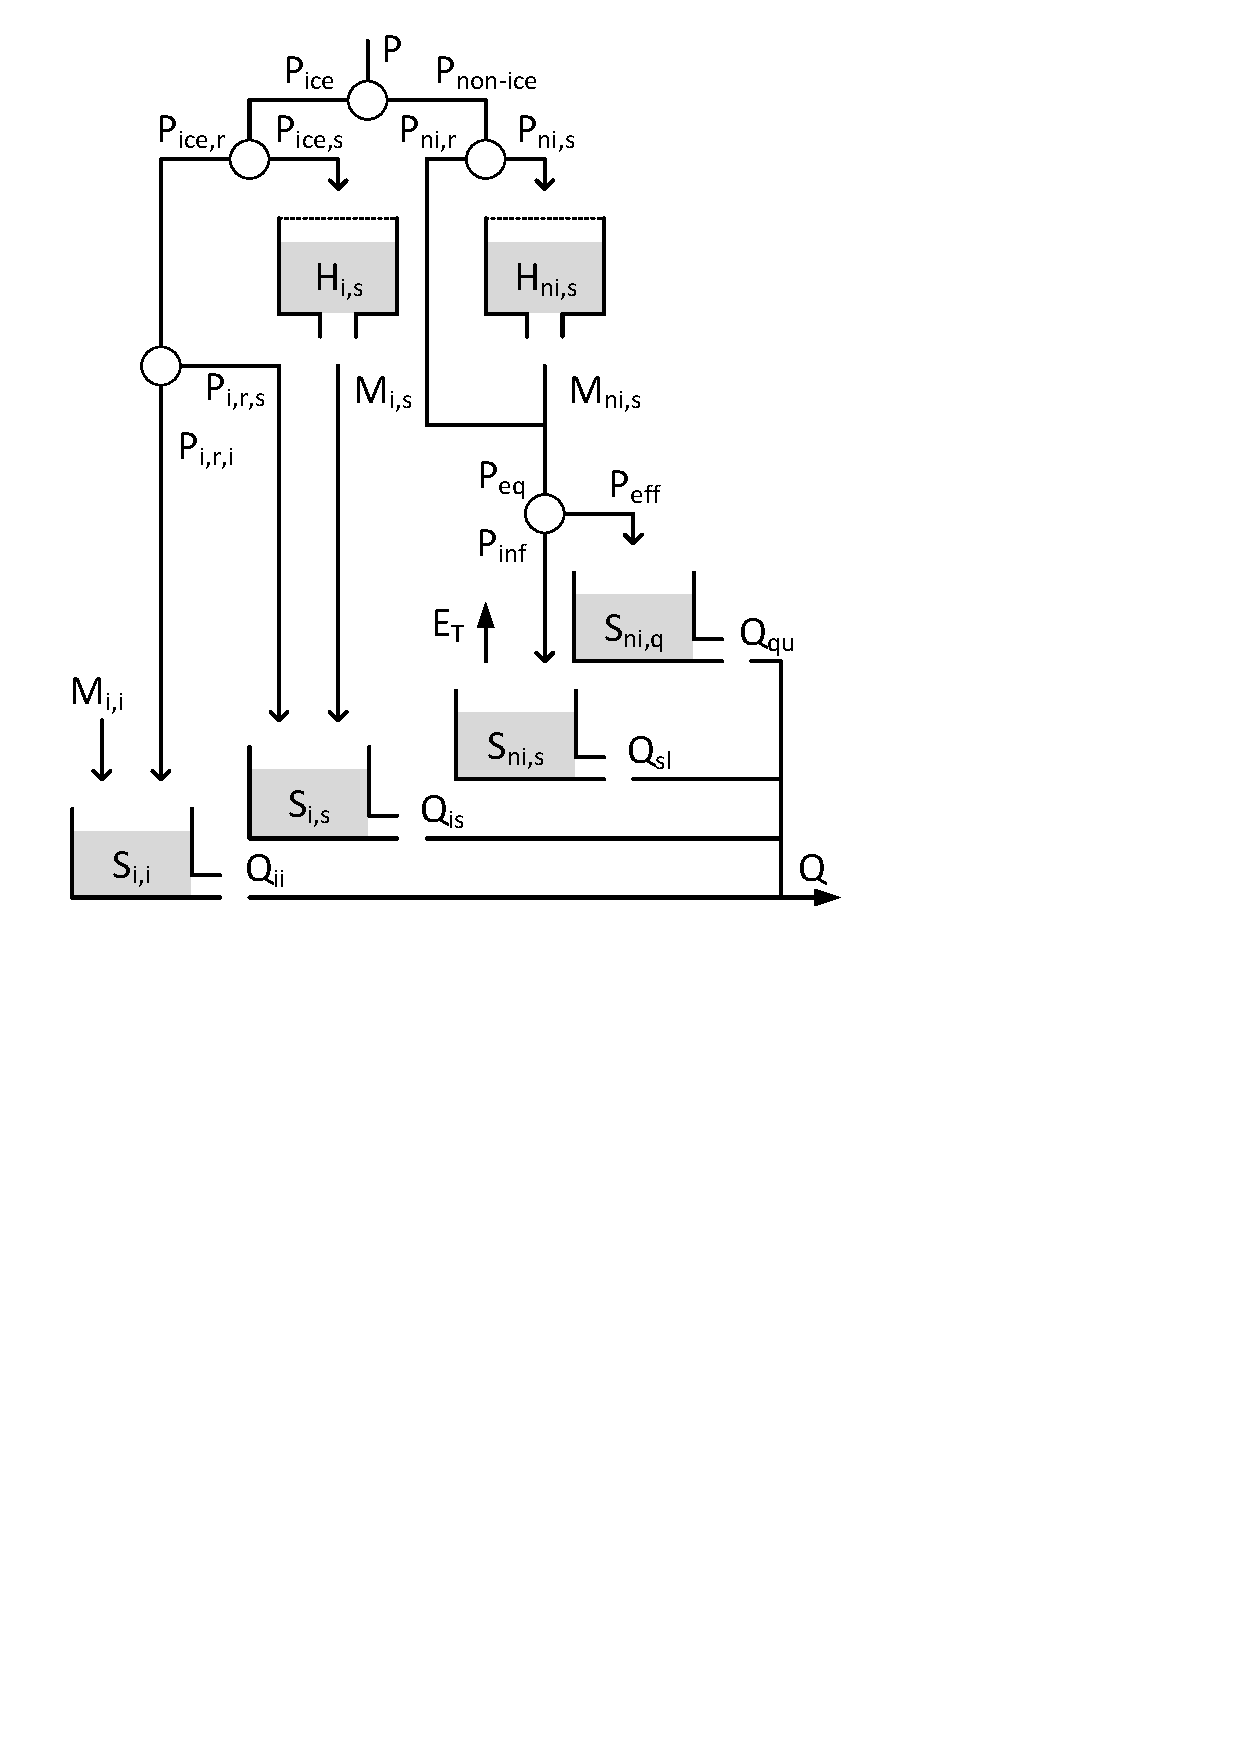
\includegraphics[trim=1cm 14cm 7cm 1cm,width=7cm,keepaspectratio]{./files/43_schematic.pdf}
\caption{Structure of the GSM-SOCONT model} \label{fig:43_schematic}
\end{wrapfigure}

\begin{align}
	\frac{dH_{i,s}}{dt} &= P_{ice,s} - M_{i,s}\\
	P_{ice,s} &= \begin{cases}
		P_{ice}, &\text{if } T \leq T_0 \\
		0, & \text{otherwise} \\
	\end{cases} \\
	P_{ice} &= f_{ice}*P \\
	M_{i,s} &= \begin{cases}
		a_{snow}(T-T_m), &\text{if } T > T_m \\
		0, &\text{otherwise} 
	\end{cases} 
\end{align}

Where $H_{i,s}$ [mm] is the current storage in the snow pack, refilled by precipitation-as-snow $P_{ice,s}$ $[mm/d]$ and depleted by melt $M_{i,s}$ $[mm/d]$.
$P_{ice,s}$ occurs only when the temperature $T$ $[^oC]$ is below a threshold temperature for snowfall $T_0$ $[^oC]$.
$P_{ice}$ is the fraction $f_{ice}$ [-] of precipitation $P$ $[mm/d]$ that falls on the ice-covered part of the catchment.
$M_{i,s}$ uses a degree-day-factor $a_{snow}$ $[mm/^oC/d]$ to estimate snow melt if temperature is above a threshold for snow melt $T_s$ $[^oC]$.

} % end of wrapfigure fix

\begin{align}
	\frac{dS_{i,s}}{dt} &= M_{i,s} +P_{i,r,s,} -Q_{is}\\
	P_{i,r,s} &= P_{ice,r}, \quad \text{if } H_{i,s} > 0 \\
	P_{ice,r} &= \begin{cases}
		P_{ice}, &\text{if } T > T_0 \\
		0, & \text{otherwise} \\
	\end{cases} \\
	Q_{is} &= k_s*S_{i,s}
\end{align}
  
Where $S_{i,s}$ [mm] is the current storage in the snow-water routing reservoir, refilled by snow melt $M_{i,s}$ $[mm/d]$ and rain-on-snow $P_{ice,s}$ $[mm/d]$, and drained by runoff $Q_{is}$.
$P_{i,r,s}$ occurs only if the current snow pack storage is above zero.
$P_{ice,r}$ is precipitation-as-rain that occurs only if the temperature is above a snowfall threshold $T_0$.
$Q_{is}$ has a linear relation with storage through time parameter $k_s$ $[d^{-1}]$.

\begin{align}
	\frac{dS_{i,i}}{dt} &= M_{i,i} +P_{i,r,i,} -Q_{ii}\\
	P_{i,r,i} &= P_{ice,r}, \quad \text{if } H_{i,s} = 0 \\
	M_{i,s} &= \begin{cases}
		a_{ice}(T-T_m), &\text{if } T > T_m ~\&~ H_{i,s} = 0 \\
		0, &\text{otherwise} \\
	\end{cases}  \\
	Q_{ii} &= k_i*S_{i,i}
\end{align}

Where $S_{i,i}$ [mm] is the current storage in the ice-water routing reservoir, refilled by glacier melt $M_{i,i}$ $[mm/d]$ and rain-on-ice $P_{ice,i}$ $[mm/d]$, and drained by runoff $Q_{ii}$ $[mm/d]$.
Both $M_{i,i}$ and $P_{ice,i}$ are assumed to only occur once the snow pack $H_{i,s}$ is depleted.
$M_{i,i}$ uses a degree-day-factor $a_{ice}$ $[mm/^oC/d]$ to estimate glacier melt. 
Ice storage in the glacier is assumed to be infinite.
$P_{ice,r,i}$ is equal to $P_{ice,r}$ if $H_{i,s} = 0$.
$Q_{ii}$ has a linear relation with storage through time parameter $k_i$ $[d^{-1}]$.

\begin{align}
	\frac{dH_{ni,s}}{dt} &= P_{ni,s} - M_{ni,s}\\
	P_{ni,s} &= \begin{cases}
		P_{non-ice}, &\text{if } T \leq T_0 \\
		0, & \text{otherwise} \\
	\end{cases} \\
	P_{non-ice} &= (1-f_{ice})*P \\
	M_{ni,s} &= \begin{cases}
		a_{snow}(T-T_m), &\text{if } T > T_m \\
		0, &\text{otherwise} 
	\end{cases} 
\end{align}

Where $H_{ni,s}$ [mm] is the current snow pack storage on the non-ice covered fraction $1-f_{ice}$ [-] of the catchment, which increases through snowfall $P_{ni,s}$ $[mm/d]$ and decreases through snow melt $M_{ni,s}$ $[mm/d]$.
Both fluxes are calculated in the same manner as those on the ice-covered part of the catchment (fluxes $P_{ice,s}$ and $M_{ice,s}$).

\begin{align}
	\frac{dS_{ni,s}}{dt} &= P_{inf} - E_T - Q_{sl}\\
	P_{inf} &= P_{eq} -P_{eff} \\
	P_{eff} &= P_{eq}\left(\frac{S_{ni,s}}{A}\right)^y \\	
	P_{eq} &= M_{ni,s} + P_{ni,r} \\
	E_T &= E_p\left( \frac{S_{ni,s}}{A}\right)^x \\
	Q_{sl} &= k_{sl}S_{ni,s}
\end{align}

Where $S_{ni,s}$ [mm] is the current storage in soil moisture, refilled by infiltrated precipitation $P_{inf}$ $[mm/d]$ and drained by evapotranspiration $E_T$ $[mm/d]$ and slow flow $Q_{sl}$ $[mm/d]$.
$P_{inf}$ depends on the effective precipitation $P_{eff}$. 
$P_{eq}$ is the total of snow melt $M_{ni,s}$ and precipitation-as-rain $P_{ni,r}$ $[mm/d]$.
$P_{ni,r}$ is calculated in the same manner as $P_{i,r}$ (equation 7).
$E_T$ is a fraction potential evapotranspiration $E_p$ $[mm/d]$, calculated using $A$ and non-linearity parameter $y$ [-].
$Q_{sl}$ has a linear relation with storage through time parameter $k_{sl}$ $[d^{-1}]$.

\begin{align}
	\frac{dS_{ni,q}}{dt} &= P_{eff} - Q_{qu}\\
	Q_{qu} &= \beta S_{ni,q}^{5/3}
\end{align}

Where $S_{ni,q}$ [mm] is the current storage in the direct runoff reservoir, refilled by effective precipitation $P_{eff}$ $[mm/d]$ and by quick flow $Q_{qu}$ $[mm/d]$.
$Q_{sl}$ has a non-linear relation with storage through time parameter $\beta$ $[mm^{4/3}/d]$ and the factor $5/3$.
Total flow:

\begin{align}
	Q &= Q_{qu}+Q_{sl}+Q_{is}+Q_{ii}
\end{align}

\newpage
\subsubsection{Parameter overview}
% Table generated by Excel2LaTeX from sheet 'Sheet1'
\begin{table}[htbp]
  \centering
    \begin{tabular}{lll}
    \toprule
    Parameter & Unit  & Description \\
    \midrule
    $f_{ice}$ & $-$   & Fraction of area with ice cover \\
    $T_0$ & $^oC$ & Threshold temperature for snowfall \\
    $a_{snow}$ & $mm~^oC^{-1}~d^{-1}$ & Degree-day factor for snowmelt \\
    $T_m$ & $^oC$ & Threshold temperature for snowmelt \\
    $k_s$ & $d^{-1}$ & Runoff coefficient \\
    $a_{ice}$ & $mm~^oC^{-1}~d^{-1}$ & Degree-day factor for ice melt \\
    $k_i$ & $d^{-1}$ & Runoff coefficient \\
    $A$   & $mm$  & Maximum soil moisture storage \\
    $x$   & $-$   & Evaporation non-linearity \\
    $y$   & $-$   & Quick runoff non-linearity \\
    $k_{sl}$ & $d^{-1}$ & Runoff coefficient \\
    $\beta$ & $MM^{4/3}~d^{-1}$ & Runoff coefficient \\
    \bottomrule
    \end{tabular}%
  \label{tab:addlabel}%
\end{table}%
